\documentclass[crop,tikz]{standalone} 
\usepackage{tikz, amsmath, amssymb, graphicx} 

\usetikzlibrary{positioning, shapes.geometric} 

\begin{document} 

\begin{tikzpicture}


\node[inner sep=0pt] (sim:0.05) at (0,0) {
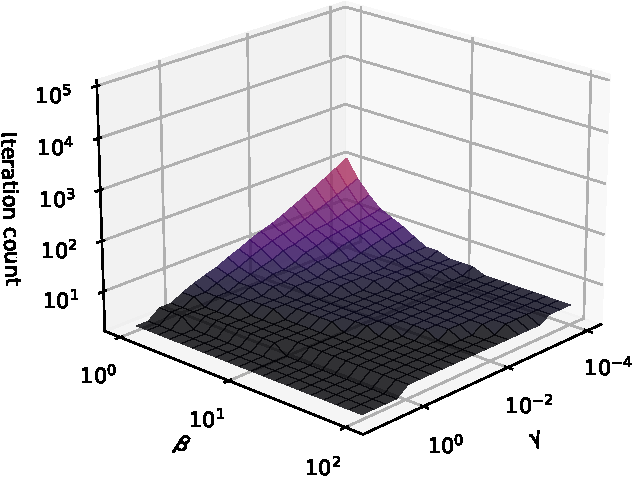
\includegraphics[width=0.5\textwidth, angle=-1]{SIM: m=0.05.pdf}
};

\node[inner sep=0pt] (cgm:0.05) at (6.5,0) {
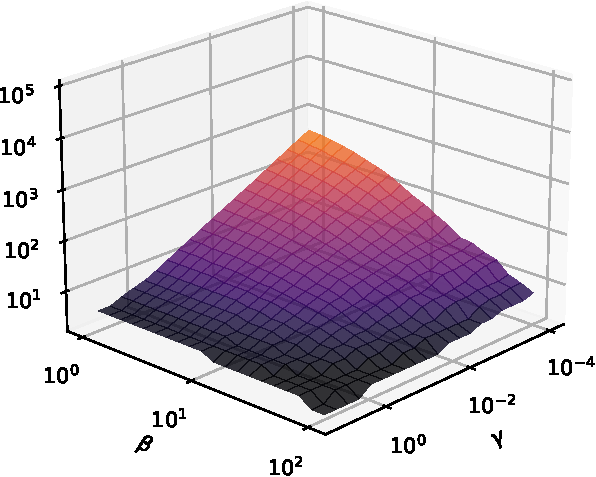
\includegraphics[width=0.5\textwidth, angle=-3]{CGM: m=0.05.pdf}
};

\node[inner sep=0pt] (sim:0.05) at (0,-5) {
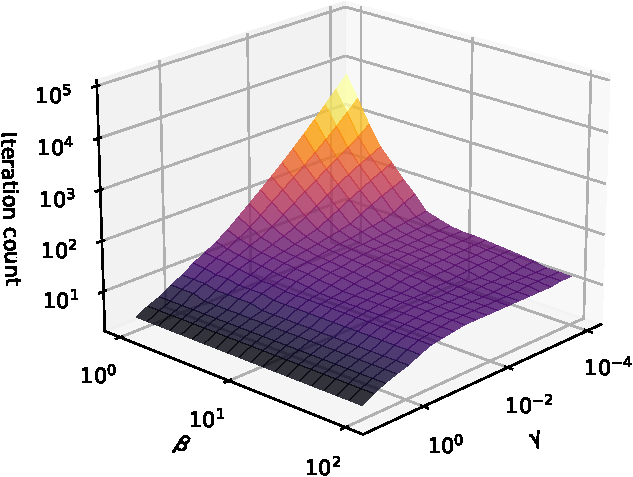
\includegraphics[width=0.5\textwidth, angle=-1]{SIM: m=0.5.pdf}
};

\node[inner sep=0pt] (cgm:0.05) at (6.5,-5) {
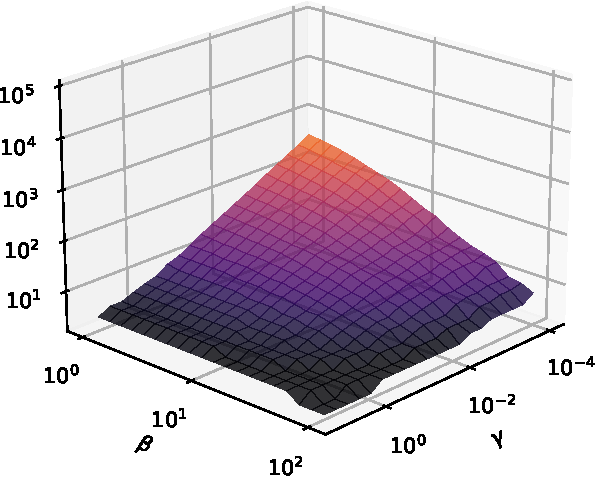
\includegraphics[width=0.5\textwidth, angle=-3]{CGM: m=0.5.pdf}
};

\node[inner sep=0pt] (sim:0.05) at (0,-10) {
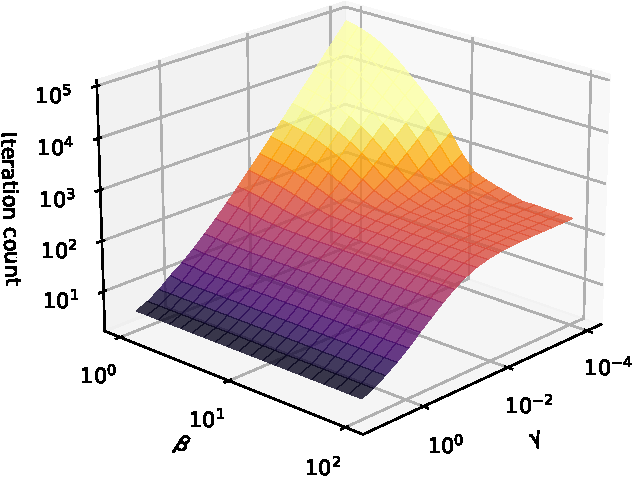
\includegraphics[width=0.5\textwidth, angle=-1]{SIM: m=0.95.pdf}
};

\node[inner sep=0pt] (cgm:0.05) at (6.5,-10) {
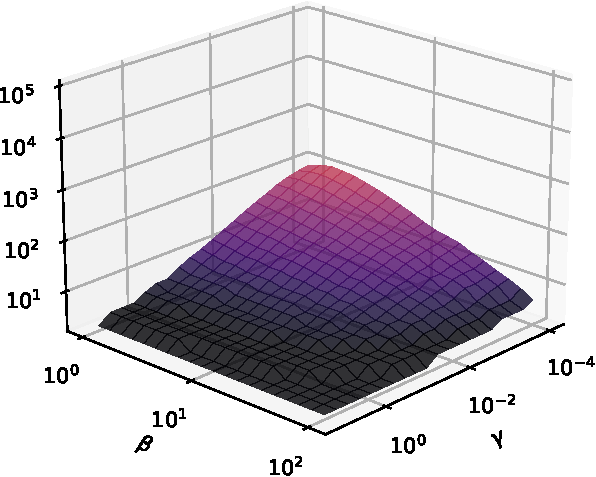
\includegraphics[width=0.5\textwidth, angle=-2]{CGM: m=0.95.pdf}
};

 

\draw (0.25,2.7) node {SIM};
\draw (6.8,2.7) node {CGM};

\draw (-4.2,0.3) node {$m=0.05$};
\draw (-4.2,-4.7) node {$m=0.5$};
\draw (-4.2,-9.7) node {$m=0.95$};


\end{tikzpicture}
\end{document} 
